\documentclass[11pt]{article}
\usepackage[margin=1in]{geometry}
\usepackage[numbers,sort&compress,round]{natbib}
\usepackage[utf8]{inputenc}
\usepackage[T1]{fontenc}
\usepackage{lmodern}
\usepackage{hyperref}
\usepackage{url}
\usepackage{booktabs}
\usepackage{amsfonts}
\usepackage{amsmath}
\usepackage{amssymb}
\usepackage{nicefrac}
\usepackage{microtype}
\usepackage{xcolor}
\usepackage{graphicx}
\usepackage{float}
\usepackage{enumitem}
\graphicspath{{figures/}}

% ============================================================
% Nature Computational Science -- ARTICLE format
% Untitled Introduction -> Results -> Discussion -> Methods (end)
% Main text target <= 3,500 words; abstract <= 200 words.
% Comprehensive version (all experiments, honest negatives): paper_nips_SUBMISSION_v11.8 (-> Supplementary).
% ============================================================

\title{Generating behaviour-equivalent parameters for whole-organism simulators from tracking video}

\author{
 Chenxi He \\
 Department of Engineering, University of Cambridge \\
 Cambridge CB2 1PZ, United Kingdom \\
 \texttt{ch2067@cam.ac.uk}
}

\date{}

\begin{document}
\maketitle

\begin{abstract}
\noindent
Mechanistic whole-organism simulators of \emph{Caenorhabditis elegans} and \emph{Drosophila} turn connectomes and biophysics into testable models of behaviour, but each is governed by hundreds to thousands of internal parameters normally fixed by invasive physiology---electrophysiology, calcium imaging, electromyography---out of reach for most laboratories and most species. We show these parameters can instead be generated from ordinary tracking video. PGOB (Parameter Generation by Observed-Behaviour) casts calibration as a behaviour-only inverse problem: one loss, one cross-simulator behavioural evaluator, and an interchangeable inference back-end (stochastic search, an evolution strategy, or an amortized neural posterior) generate, from kinematics alone, parameter sets that reproduce a simulator's behaviour, together with a Jacobian that attributes any residual mismatch to a specific mechanism. Across four published simulators spanning two species the same formulation generates behaviour-equivalent parameters from an uninformative start; where a simulator carries a genuine real reference, PGOB reproduces the simulator's own target more tightly than two real animals differ from each other (recovered-to-target $0.71$ vs real-to-real $1.98$ on the worm), while the deposited default lies an order of magnitude further from real biology. The generated parameter distributions transfer as same-species priors and carry a modest prospective signal for $43$ held-out mutant strains, consistent with species-level structure rather than arbitrary curve-fit residue. PGOB offers a route to calibrating whole-organism models where invasive recording is impossible.
\end{abstract}

% ===================== INTRODUCTION (untitled) =====================
Mechanistic, whole-organism simulators have become a central tool for turning connectomes and biophysics into testable models of how brains and bodies generate behaviour \citep{wang2025baaiworm,shlizerman2025modworm,vaxenburg2025flybody,wangchen2024neuromechfly}. Every such simulator, however, is governed by hundreds to thousands of internal biophysical parameters, and inferring those hidden parameters from observable outputs is the classical inverse problem of systems identification \citep{villaverde2014reverse,spall2003introduction}. In current practice they are pinned by direct, invasive physiology---intracellular electrophysiology, two-photon imaging, electromyography---that most laboratories cannot perform and that, for many species, cannot be performed at all. This bottleneck is general to the field: a simulator's parameters are typically fixed by one or two source studies, almost no calibrated set has been tested \emph{prospectively} on biology it never saw, and any laboratory or species for which only movement can be recorded is, in effect, locked out of the very simulators built to model it. The settings where the bottleneck bites hardest---organisms with no historical physiology, endangered animals, preparations that cannot be patched or imaged---are exactly those where invasive recording is hardest, yet whose behaviour can still be filmed.

Here we show this lock can be opened with tracking video alone. Given a published simulator and nothing but the externally observed kinematic trajectory of a real animal, PGOB (Parameter Generation by Observed-Behaviour) generates a working set of simulator parameters and returns a Jacobian sensitivity map that attributes any residual behavioural mismatch to a specific simulator mechanism. PGOB is a \emph{formulation} of the behaviour-only inverse problem, not a new optimiser: the inference engine that searches parameter space---stochastic approximation, an evolution strategy, or amortized simulation-based inference \citep{cranmer2020frontier}---is an interchangeable back-end. The same formulation, the same cross-simulator behavioural evaluator and the same engine stack run on every model we test; the one component that adapts is the initialisation, which is dimension-dependent and itself a reported finding. The contribution is therefore the behaviour-only inverse-problem formulation together with a cross-simulator evaluator and a residual-to-mechanism attribution map: unlike single-circuit system identification \citep{izquierdo2013connecting} it operates at whole-organism scale across multiple published simulators, and unlike simulation-based inference fitted to one model it is deliberately engine- and simulator-agnostic. Because the starting point is drawn independently of the unknown optimum, obtaining a working simulator from motion is parameter \emph{generation}, not a small correction to an already-good guess. We demonstrate PGOB on two \emph{C.~elegans} simulators (BAAIWorm \citep{wang2025baaiworm}, modWorm \citep{shlizerman2025modworm}) and two \emph{Drosophila} simulators (flybody \citep{vaxenburg2025flybody}, FlyGym \citep{wangchen2024neuromechfly}); Table~\ref{tab:claimmap} summarises which experiment, metric and test underpins each finding that follows.

% ===================== RESULTS =====================
\section*{Results}

\begin{table}[h]
\centering\scriptsize
\caption{\textbf{Each main finding maps to a single experiment, primary metric and statistical test.} On the two simulators with a genuine real reference the unit-free $G{=}D_1/D_2$ (recovery-to-target as a multiple of the real animal-to-animal spread) is cross-simulator comparable (Table~\ref{tab:hierarchy}). Secondary diagnostics are reported once where they arise and are not cross-row comparable. The held-out mutant prediction is corroborating biological evidence.}
\label{tab:claimmap}
\begin{tabular}{p{3.0cm}p{2.7cm}p{2.9cm}p{1.9cm}p{2.5cm}}\toprule
Finding & Experiment & Primary metric & Test & Result \\\midrule
Behaviour-equivalent generation from a random start & three-segment (FlyGym) $+$ PGOB-sim $\theta^*$ & generation fraction; $\mathrm{rel}_\theta$ to sim $\theta^*$ & bootstrap CI & FlyGym $94.9\%$; modWorm $\mathrm{rel}_\theta{=}0.009$ \\
Recovery tighter than real animal-to-animal spread & three-distance hierarchy & $D_1$ (recovered$\to$sim) vs $D_2$ (real$\to$real) & $1000/1000$ bootstrap & BAAIWorm $0.71{<}1.98$; flybody $0.20{<}0.42$ \\
Improves on the deposited parameters & PGOB-vs-baseline parity (Initialized=capability; expert default=deployment) & per-obs.\ $W_1$ improved frac. & Mann--Whitney $+$ Holm & capability FlyGym $8/10$; deployment BAAIWorm $7/10$, flybody $0/9$ (null) \\
Engine-agnostic & NPE-MAF, same task & posterior-predictive behaviour reproduction & SBC $+$ held-out NLL & modWorm $1.4{\times}10^{-3}$; FlyGym rel $0.018$ \\
Transferable species structure & same-species prior transfer & held-out starts improved & one-sided Wilcoxon & $13/16$, $p{=}0.025$ \\
Prospective mutant signal & 43-strain LOSO & LOSO Spearman vs.\ shuffle & paired Wilcoxon & $0.684$ vs.\ $0.527$, $p{\approx}0.009$ \\
Biology-grounded, not an arbitrary fit & cross-species generation matrix & target conditions reached; feature deviation & descriptive & within-phylum all reached ($<0.4\%$); cross-species $6/8$ at $0$ ($87$--$93\%$) \\
Parameter- not dynamics-space & Jacobian attribution & per-axis $|\partial M/\partial\theta|$ & descriptive & reversals $\to$ \texttt{syn} \\\bottomrule
\end{tabular}
\end{table}

Each finding below is tied to a single experiment, primary metric and statistical test (Table~\ref{tab:claimmap}); the unit-free $G{=}D_1/D_2$ is the one quantity readable the same way on every simulator, and every other number answers one specific question where it appears.

We begin from the basic question of whether parameters can be generated from behaviour alone, and place every generation on a single anchored axis that runs from a random start, through the generated parameters, to the simulator's expert default and finally to real biology. On a FlyGym \emph{Drosophila} walker whose start is a fully randomised, frequently non-walking actuator-gain vector---one that fails to walk at all in $8/20$ rollouts---the generated parameters close $94.9\%$ of the random-to-expert behavioural distance (forward speed $98.7\%$, lateral speed $90.4\%$), landing within $1.3\%$ of the expert ground truth (Fig.~\ref{fig:hero}). Because the start carries no information about the optimum, this is generation, not a small correction: behaviour-only video is enough to drive an uncalibrated simulator onto a working set of parameters.

Where a simulator's own ground-truth target $\theta^{*}$ is known we can ask the sharper question of whether the recovered \emph{parameters}, not merely the behaviour, are correct, because here the answer can be checked directly in parameter space. On the $30$-d modWorm, PGOB recovers $\theta^{*}$ to relative error $\mathrm{rel}_\theta{=}0.009$---the tightest of any simulator---with flybody at $0.115$ ($515$-d) and FlyGym at $0.365$. We stress that this $\theta^{*}$ is the simulator's \emph{internal} target, not a measurement of the animal's physiology; for real biology, where no parameter ground truth exists, the claim is restricted to behaviour-equivalent parameter sets. What we therefore learn is that the procedure does not merely land on some behaviourally-equivalent point: where the truth is known to us, it is reached, and the gap between modWorm's near-exact recovery and the higher-dimensional simulators' looser values is itself the signature of how strongly trajectory observables constrain each parameterisation.

The most demanding test of generation is the BAAIWorm connectome, where the ``full5'' parameterisation acts not on a handful of global scales but directly on the per-element synaptic ($\approx2{,}000$), gap-junction ($\approx1{,}000$), motor-output, per-cell ion-channel and per-cell passive-membrane weight vectors, concatenated into a single several-thousand-dimensional search vector. From a fully scrambled $100\%$ start, multicondition SPSA ($60$--$140$ iterations) followed by CMA-ES and a refinement stage rebuilds this entire parameter set up to the simulator's published behaviour band: the best held-out checkpoint reaches behaviour distance $0.1199$ on the $160$-condition out-of-distribution panel, matching BAAIWorm's deposited state-of-the-art band ($0.120$--$0.125$), with the same run averaging $0.162$ over the full panel. That a connectome's worth of per-element weights can be regenerated from scrambled noise up to the model's own deposited performance shows the formulation scales past low-dimensional pilots to the parameterisations these simulators actually ship. The behaviour underlying these scalars is the \emph{C.~elegans} travelling undulation wave, whose bend-wave correlation to target rises $0.76\to1.00$ where the random start stays flat (Fig.~\ref{fig:wave}).

We next place the generation between the simulator's own target and the spread of real biology. On the two simulators carrying a genuine real reference we compute three z-scored behavioural distances on that real corpus: $D_1$ (generated$\to$the simulator's own target), $D_2$ (real$\to$real individual spread) and $D_3$ (deposited default$\to$real). The within-row ordering $D_1{<}D_2{\ll}D_3$ holds on both (Table~\ref{tab:hierarchy}); on the BAAIWorm five-scale deployment parameterisation, $D_1{=}0.71<D_2{=}1.98\ll D_3{=}21.82$ in $1000/1000$ bootstrap resamples, and on flybody $0.20<0.42\ll2.53$. The recovery to the simulator's own target is therefore tighter than the real animal-to-animal spread, while the deposited default lies an order of magnitude beyond it---the distance a calibration method exists to close.

To compare this \emph{across} simulators despite their heterogeneous references, we report the unit-free ratio $G{=}D_1/D_2$: the recovery-to-target distance expressed as a multiple of that simulator's real animal-to-animal spread. The per-observable $z$-scale appears in both numerator and denominator and cancels, so $G$ is comparable across simulators, and $G{<}1$ means the recovery to the simulator's own target is tighter than real individual variation. Both simulators with a genuine real reference satisfy $G{<}1$ (BAAIWorm $0.36$, flybody $0.48$). $G$ measures recovery tightness, not closeness to real biology; the deposited-default distances ($D_3$) are what quantify how far the shipped models sit from real.

\begin{table}[h]
\centering\small
\caption{\textbf{Three-distance hierarchy on the two simulators with a genuine real reference.} $D_1$ = generated vs the simulator's own target; $D_2$ = real animal-to-animal spread; $D_3$ = deposited default vs real. Each row is z-scored on that simulator's own real corpus, so within-row ordering $D_1{<}D_2{\ll}D_3$ is the meaningful read and absolute magnitudes are not cross-row comparable. The unit-free $G{=}D_1/D_2$ (recovery tightness relative to real spread) is cross-simulator comparable. BAAIWorm is the five-scale deployment parameterisation.}
\label{tab:hierarchy}
\begin{tabular}{lccccc}\toprule
Simulator & Species & $D_1$ (recov.$\to$sim) & $D_2$ (real$\to$real) & $D_3$ (default$\to$real) & $G{=}D_1/D_2$ \\\midrule
BAAIWorm & \textit{C.~elegans} & 0.71 & 1.98 & 21.82 & \textbf{0.36} \\
flybody walking & \textit{Drosophila} & 0.20 & 0.42 & 2.53 & \textbf{0.48} \\\bottomrule
\end{tabular}
\end{table}

The same generation can be read three ways, and doing so separates what the simulator can reach from what real biology demands. PGOB operates in three modes, none requiring electrophysiology. \emph{PGOB-sim} optimises against a simulator's own synthetic state-of-the-art target and validates framework integrity (the known $\theta^{*}$ should be generated); \emph{PGOB-real} optimises directly against real OWMD or Janelia trajectories (the scenario a behaviour-only laboratory actually faces); \emph{PGOB-hybrid} warm-starts on the simulator's own behaviour and then fine-tunes against real video (the production protocol). Each cell of Table~\ref{tab:modes_v8} is a genuine optimisation from its own randomised (or, for the high-dimensional simulators, prior-seeded) start, not a midpoint or convex blend of the endpoints, and run this way the simulators tell one consistent story. In PGOB-sim mode the procedure reproduces each simulator's own target tightly---BAAIWorm reaches a behaviour distance of $0.198$, FlyGym $3.42$, and in parameter space modWorm recovers $\theta^{*}$ to $\mathrm{rel}_\theta{=}0.009$, the tightest of any simulator. In PGOB-real mode every simulator settles at a sim$\leftrightarrow$real floor (modWorm $W_1{=}1.25$, FlyGym $52.2$), and the PGOB-hybrid warm-start lands at essentially that same floor (BAAIWorm $2.67$ vs the real arm's $2.63$, modWorm $1.32$ vs $1.25$, FlyGym $53.9$ vs $52.2$): in every case within run-to-run noise of the cold-start real fit and, if anything, marginally above rather than below it. The production warm-start therefore mainly buys faster convergence to the sim$\leftrightarrow$real floor; the held-out accuracy gain over a cold real fit is mild at best, and no arm---sim-targeted, real, or hybrid---reaches the real animal-to-animal spread. Read one channel at a time, the same generation is visible in the behaviour itself: on a single FlyGym fly the generated controller closes $94.9\%$ of the random-to-expert-controller aggregate gap ($13.30\to10.78\to10.64$, $N{=}20$/arm; the expert is the simulator's canonical gains) with the forward- and lateral-speed channels collapsing almost onto expert, while the randomised start fails to walk in $8/20$ rollouts.

\begin{table}[h]
\centering\small
\caption{\textbf{Three deployment modes $\times$ three simulators, each scored against the object it optimises.} \textbf{PGOB-sim} is scored against the simulator's own $\theta^{*}$ target behaviour (the framework-integrity yardstick); \textbf{PGOB-real}/\textbf{-hybrid} against real biology (the deployment yardstick). Values are held-out behaviour distance, comparable \emph{within} a row (one shared start and scale), not across rows. PGOB-sim reproduces the sim target tightly; PGOB-real/-hybrid settle at the sim$\leftrightarrow$real floor. $^{\dagger}$modWorm's PGOB-sim cell is the parameter-generation relative error $\mathrm{rel}_\theta{=}0.009$ (matched behaviour distance $W_1{=}3.1\times10^{-3}$), a scale-$0.1$-start point estimate; under harder starts or the neural-posterior engine the parameters are behaviour-equivalent rather than uniquely identified. These three-mode cells use the low-dimensional parameterisation; the full5 ($\approx5$k per-element) generation is reported separately against the simulator's SOTA band ($0.1199$).}
\label{tab:modes_v8}
\begin{tabular}{lccc}\toprule
Simulator & PGOB-sim $\to$ sim $\theta^{*}$ & PGOB-real $\to$ real & PGOB-hybrid $\to$ real \\\midrule
BAAIWorm   & 0.198 & 2.63 & 2.67 \\
modWorm    & $0.009^{\dagger}$ & 1.25 & 1.32 \\
FlyGym v2  & 3.42  & 52.2 & 53.9 \\\bottomrule
\end{tabular}
\end{table}

A practitioner's question is whether the generated parameters are good enough to \emph{use} in place of the expert default they would otherwise download. Optimising cold against real trajectories, behaviour-only PGOB-real reached a standardised distance-to-real on a par with the simulator's own physiologically-calibrated default (BAAIWorm recovered-to-real $21.8$ vs.\ default $21.8$; modWorm $3.29$ vs.\ $2.69$), both still beyond the real animal-to-animal spread because the substrate cannot express those channels at any parameter setting. The honest headline is therefore parity, not superiority: behaviour-only inference reaches what a physiological calibration reaches, without performing one. We keep the per-observable comparison terminologically clean. We reserve \emph{default} for a simulator's expert-calibrated, published parameters, and \emph{Initialized} for the uninformative randomised start; a test against an Initialized reference measures raw generation capability, a test against an expert default measures deployment value, and the two baseline types are never pooled or summed. Against an Initialized reference PGOB moved the per-observable Wasserstein-1 distance toward real biology on $8/10$ FlyGym observables ($+32.4\%$ mean, Holm-significant)---a capability result, since the Initialized start is deliberately weak. Against an expert default the picture is, consistently, parity rather than gain: on BAAIWorm $7/10$ observables shifted toward real but the mean OWMD-N2 change was small ($+4.17\%$), and on the already-strong flybody walking default no observable reached significance ($0/9$, all $|d|{<}0.41$). Whatever room remains for a deployment gain tracks how far the expert default already sits from the substrate's reachable behaviour: a loose default leaves room, a well-tuned one little. Both ends are observed---re-running PGOB against FlyGym's well-tuned \emph{shipped} controller gains moved $6/10$ observables toward real (aggregate $W_1$ $983.4\to52.5$), whereas flybody's expert default could not be improved on---so what behaviour-only generation reliably delivers is a parameter set as good as the expert default, obtained without any physiology (Fig.~\ref{fig:logratio}).

If PGOB is genuinely a formulation rather than a particular optimiser, swapping the inference engine should leave the generations unchanged, so we test exactly that. Replacing the black-box optimiser with an amortized neural posterior (NPE-MAF \citep{papamakarios2017maf}, \texttt{sbi} toolkit \citep{tejero2020sbi}) on the \emph{identical} setup reproduces each simulator's behaviour: posterior-predictive behaviour matches the modWorm target to mean absolute observable difference $1.4{\times}10^{-3}$, and the FlyGym posterior mean lands at $\mathrm{rel}_\theta{=}0.018$ (Fig.~\ref{fig:engine}). The two engines are complementary, not rival: on the shared $48$-d FlyGym task the optimiser returns a fast point estimate that settles on the behaviourally-equivalent set ($\mathrm{rel}_\theta{=}0.16$ to the canonical gains while matching behaviour), whereas the amortized posterior, trained once over the prior on $N{=}6{,}000$ valid simulations (modWorm $N{=}14{,}993$), pins the gains markedly tighter ($\mathrm{rel}_\theta{=}0.018$) and additionally returns a calibrated distribution that can be sampled for any new observation without re-running the optimiser. Two diagnostics confirm the back-end behaves as a well-calibrated density model rather than an ad-hoc fit. Held-out negative log-probability orders the three density estimators in the expected direction on both simulators---neural spline flow $<$ MAF $<$ mixture-density network (modWorm $46.3/49.8/51.6$; FlyGym $157.3/161.5/165.8$; lower is a better fit)---so improvements in generic density estimation carry into PGOB unchanged. Per-dimension rank-based simulation-based calibration is consistent (per-axis KS at $\alpha{=}0.05$) on $10/30$ modWorm and $22/48$ FlyGym posterior dimensions: precisely the well-identified, behaviour-sensitive axes, with the remaining dimensions the weakly-identified directions a behaviour-only observation cannot constrain---the count is therefore an honest map of what trajectories do and do not pin, not a failure (SI \S S4.13). Because the same generations emerge whether the search is run by stochastic optimisation or by a trained density model, the contribution we are reporting is the behaviour-only formulation, not the choice of optimiser, and well-understood advances in either engine carry into PGOB unchanged.

\paragraph{The generated parameter distribution carries transferable species structure.} Were the generated numbers arbitrary curve-fit residue, a distribution learned on one simulator would carry no usable structure for another. Instead, the generated parameter \emph{distribution} transfers as a same-species soft prior: a BAAIWorm-derived per-biophysical-class prior (per-class mean and spread, not raw values) outperforms modWorm's own default initialisation on $13/16$ held-out starts (mean held-out distance $3.37\to2.29$; one-sided Wilcoxon $p{=}0.025$; SI \S S4.6), and a FlyGym$\to$flybody self-prior lowers the CMA-ES loss $9.3\times$ (default $0.01085\to0.001166$, $515$-d). This matters because high-dimensional embodied controllers are acutely start-sensitive: flybody from a pure random scale-$1$ start sits at relative error $1.061$ with CMA-ES near-stationary, and FlyGym at the same start crashes to a MuJoCo NaN and cannot be optimised at all---so a prior that rescues an otherwise-stalled generation reflects genuine structure, not arithmetic.

Two details fix the mechanism by which this structure transfers, and are themselves the reason there is no universal-best initialisation (a dimension-adaptive decision tree, SI \S S5.1). First, only the \emph{soft} prior transfers: mapping the per-biophysical-class coefficient of variation onto the per-axis CMA-ES step size leaves the optimiser free to walk away from any mis-pinned coordinate, whereas a \emph{hard} linear-projection initialisation that pins the parameters outright gives \emph{negative} transfer ($\mathrm{rel}_\theta{=}-0.127$, worse than a random start), because it lands the search in a basin it cannot escape. Second, the class correspondence is biophysically informed rather than exact (\texttt{gap}$\to$gap-junction, synaptic$\to$synaptic, membrane$\to$passive, ion$\to$ion, muscle$\to$motor-output; SI \S S4.6), so the transferred quantity is the \emph{shape} of the species-level parameter distribution, not its raw coordinates. Arbitrary numbers tuned to one simulator could not survive being re-expressed as a per-axis spread on a different simulator's parameterisation; the species-specific distribution does.

\paragraph{The generated structure generalises across laboratories.} A second, independent test of whether the generated parameters track biology rather than one acquisition paradigm is cross-laboratory transfer. Comparing Schafer-OWMD (Cambridge MRC LMB, $N{=}200$ windows) against Brown-Tierpsy (Imperial College London, $N{=}52$ windows) on six simulator-agnostic centreline observables under leave-one-laboratory-out gives a median cross/within Wasserstein-1 ratio of $2.80\times$. Crucially, every pattern-level observable---the kind PGOB actually targets---is partially universal ($<3\times$): spectral entropy $1.75\times$, body curvature $2.48\times$, head--tail orientation $2.64\times$, and left--right phase coupling $2.96\times$; only absolute, paradigm-dependent observables such as stride frequency ($3.90\times$) and length-normalised speed ($6.10\times$) exceed it. Training jointly on both laboratories narrows the held-out-laboratory gap, lowering the cross/within ratio from $3.77$ (single-laboratory) to $2.33$ (joint), a $1.62\times$ improvement, with left--right phase coupling identified as the laboratory-invariant axis. The generated behavioural structure thus generalises beyond the single cohort it was fitted to.

\paragraph{The generated sensitivities extrapolate prospectively to held-out biology.} From the N2-generated $\theta^{*}$, the Jacobian predicts behavioural deviation on $43$ held-out \emph{C.~elegans} mutant strains never seen during fitting \citep{yemini2013openworm}. Leave-one-strain-out prediction gives mean Spearman $\bar\rho{=}0.684$ (median $0.80$, $41/43$ strains $\rho{>}0$) versus a strain-shuffle null $\bar\rho_0{=}0.527$ (paired Wilcoxon $p{\approx}0.009$; SI \S S4.3)---a modest but real prospective signal that the generated parameters carry information beyond the population-average mutant direction. Predictability stratifies by molecular mechanism in a way that matches the Jacobian's active subspace: the top-predictable strains ($\rho{=}1.0$) are neuromodulator, G-protein and peptidergic mutants (\emph{egl-30}, \emph{egl-8}, \emph{ser-1}, \emph{flp-1}, \emph{flp-18}), whose lesions act through the synaptic, gap-junction and motor-output scales the Jacobian spans, whereas the weakest strains (\emph{unc-104}, \emph{unc-1}; $\rho{\sim}0.2$, still positive) are structural and axonal-transport mutants whose effect lies outside that subspace. The signal survives the pre-registered full feature set ($\bar\rho{=}0.525$ vs.\ shuffle $0.338$, $\Delta{=}{+}0.187$, $27/28$ strains $\rho{>}0$; SI \S S4.3) and a second worm laboratory; the full-feature confirmation runs on the $28$ of $43$ strains whose Yemini features were retrievable from source. A further unpaired consistency check points the same way: although no neural signal enters the loss, the generated BAAIWorm simulator's internal whole-brain dynamics agree with independent Kato-2015 whole-brain calcium imaging \citep{kato2015global} on $2/4$ population-level distributional invariants (pairwise correlation magnitude $|\mathrm{corr}|{=}0.21$ and slow-band spectral fraction $0.74$ both fall in the simulator's range; PCA dimensionality and autocorrelation time constant differ). We present these as corroborating evidence, not proof: the behaviour-only inverse problem is underdetermined, so whether the generated parameters lie on the biological parameter manifold remains for future work.

\paragraph{Generation fails across species, as a biology-grounded method should.} If PGOB were an arbitrary curve-fitter it would bend any simulator onto any target; instead, generation succeeds only when the substrate can physically express the target behaviour. Asked to reproduce a target from its own phylum, every simulator reaches it (worm-simulator$\leftrightarrow$worm-target and fly-simulator$\leftrightarrow$fly-target: all $5/5$--$6/6$ conditions reached, residual feature deviation $<0.4\%$). Asked to reproduce a target from the \emph{other} phylum---a \emph{C.~elegans} simulator driven toward \emph{Drosophila} walking, or a fly simulator toward worm chemotaxis---generation breaks down: six of eight cross-species pairs reach $0$ of their target conditions at $87$--$93\%$ residual feature deviation, and even the two least-mismatched pairs (a fly simulator approximating worm forward crawling) reach only $3/6$ conditions at $59\%$ deviation---an order of magnitude worse than within-phylum fitting. That the method can be \emph{falsified} this way---that it cannot manufacture an arbitrary behaviour from the wrong body---is positive evidence that the parameters it generates are constrained by the simulator's biology, not by the flexibility of the search.

\paragraph{Scope: a parameter-space generation framework.} A controlled ablation makes the framework's scope precise and is itself a clean positive result (Fig.~\ref{fig:ablation}). We applied the identical SPSA pipeline to compensate three families of injected corruption. On BAAIWorm \emph{parameter}-space corruption (additive Gaussian weight noise at $0/5/20/50\%$ plus a $30\%$ index-shuffle), generation succeeds on \emph{all $30/30$ cells} (mean drop $\Delta L/L_0{=}-29.4\%$ over the full $L_0$--$L_5$ sweep); a targeted re-run of the three lowest corruption levels at $n{=}10$ seeds sharpens the low-severity end into a clean monotone gradient ($L_0{=}0.068$, $L_1{=}0.071$, $L_2{=}0.101$), so generated-parameter quality degrades smoothly as corruption deepens. In contrast, \emph{dynamics}-space corruption cannot be repaired: injecting modWorm state noise collapses observable closeness from $0.9999$ to $0.30$ while the optimiser saturates, and stressing the FlyGym integrator diverges it on $4/6$ levels, leaving no usable forward model. The asymmetry is mechanistic, not optimiser-side: PGOB is a parameter-space generation framework with a clearly stated scope, not a dynamics-space repair tool. Consistent with the same premise, a pre-registered neural-ablation control finds that adding internal neural signal to the loss yields no detectable gain over the pure-trajectory loss (paired difference $+0.0030$, Cohen's $d{=}0.14$, Wilcoxon $p{=}0.734$), underwriting the behaviour-only design.

\paragraph{Residuals localise to a named mechanism.} At the generated $\theta^{*}$, a $5\times5$ finite-difference Jacobian $|\partial M/\partial\theta|$ ($\varepsilon{=}2\%$) maps each behavioural residual onto the parameter group that controls it. The worst per-metric residual is worm reversals, $=0.261$, and its $|J|$ row is dominated by the synaptic axis at $|J|{=}2.47$---roughly $50\times$ the next-largest entry---so the residual routes cleanly to \texttt{syn} (Fig.~\ref{fig:hero}c). This points to a specific simulator-side component---BAAIWorm's reversal generator is a fixed synaptic weight matrix---as where the residual concentrates. The attribution map thus turns each residual, axis by axis, into a named simulator parameter group rather than a single aggregate distance.

% ===================== DISCUSSION =====================
\section*{Discussion}
PGOB turns simulator calibration into a behaviour-only inverse problem and shows, across four published whole-organism simulators and two species, that ordinary tracking video suffices to generate behaviour-equivalent parameter sets from an uninformative start; where a genuine real reference exists, the recovery to the simulator's own target is tighter than real animal-to-animal variation, while the deposited default lies far beyond it. The contribution is the formulation, the cross-simulator behavioural evaluator and the residual-to-mechanism Jacobian; the inference engine---black-box optimiser or amortized neural posterior---is an interchangeable back-end, so well-understood advances in either carry over directly. Several converging findings indicate the generated numbers carry biological, not merely numerical, structure: a generated distribution transfers as a same-species prior that rescues an otherwise-stalled generation, the generated sensitivities extrapolate prospectively to $43$ held-out mutant strains, the generated behavioural structure generalises across two laboratories, and the simulator's internal dynamics agree with independent whole-brain imaging on half of four population-level invariants despite receiving no neural supervision. Because the inverse problem is underdetermined, we frame these as corroboration rather than proof that the values are the biological ones; whether they lie on the biological parameter manifold is a question we pose for future work.

Three results must be read separately and are never allowed to borrow strength from one another. The first is \emph{capability}: from an uninformative or Initialized start PGOB generates behaviour-equivalent parameters and, where the simulator's own target $\theta^{*}$ is known, recovers it tightly. We are explicit that this sim-recovery is a \emph{controlled} inverse problem---the candidate and target rollouts share the same start state, episode length and food/stimulus schedule---so on its own it does not establish that parameters can be inferred when the inputs that drove the behaviour are unknown. \emph{Real deployment} is the test that does: optimised cold against real trajectories, where the stimuli, gradients and internal drives behind the animal's path are entirely unobserved, PGOB still infers a working parameter set from kinematics alone and attains a standardised distance-to-real comparable to the simulator's \emph{own physiologically-calibrated expert default} (BAAIWorm $21.8$ vs.\ $21.8$; modWorm $3.29$ vs.\ $2.69$). We do \emph{not} claim to surpass that default---an extended-budget hybrid fine-tune moves held-out fit by only $-1.1\%$, $-5.5\%$ and $-2.0\%$, and no arm reaches within the real individual spread, because the expert default already sits at the simulator's sim$\leftrightarrow$real ceiling, which no parameter choice within the substrate can pass. The claim is the one a behaviour-only laboratory actually needs: for a new simulator or species with \emph{no} measured physiology, PGOB attains---from observed movement under unknown driving conditions---the level a direct physiological calibration would reach, without any electrophysiology. The Initialized-start rescue results quantify capability, not this deployment parity, and we never use one to argue the other. Where the ceiling bites, the contribution shifts from closing the gap to localising it: the attribution map names the mechanism a simulator would have to add. The route past the invasive-measurement bottleneck is accordingly a route to obtaining working, behaviour-equivalent parameters---matching physiological calibration without performing it---and to diagnosing where a simulator falls short, not to surpassing physiology in closeness to real. Within that scope, composing behaviour-only generation with same-species prior transfer suggests a route to populating behaviourally-grounded digital organisms at scale from tracking video, without electrophysiology.

Three boundaries delimit the method's scope, and in each the attribution map turns the limit into a diagnosis rather than a bare gap. First, the reachable fidelity is a property of the deposited simulator, not of PGOB: the modWorm $30$-d Cook-ODE substrate cannot express the high-order eigenworm-variance modes that distinguish real worms, so even its expert arm cannot reach those channels (where it can, PGOB closes the gap exactly, e.g.\ matching OWMD's \texttt{active\_frac} of $0.4975$); and, second, the flybody walk-imitation benchmark is a single MoCap-locked task whose trajectory observables carry no extractable parameter signal, placing it outside the scope of trajectory-only generation (its initialisation signal instead lives in loss space, where the same-species prior still gives a $9.3\times$ gain). In both cases PGOB names which mechanism would have to be added rather than reporting only that a gap exists, converting calibration into a simulator-side debugging task. Third, the behaviour-only inverse problem is underdetermined, so the generated parameters are behaviour-equivalent and need not be the unique biological ones; and the same-species prior transfer demonstrated here uses a biophysically-informed dimension map between two simulators of one species, leaving open whether a comparable prior helps across more distantly related body plans.

The payoff is largest exactly where the bottleneck bites hardest. Because the formulation is simulator- and engine-agnostic and consumes only externally observable behaviour, it can in principle be pointed at organisms the bottleneck excludes outright: species with no historical electrophysiology, endangered animals that cannot be sacrificed for patch-clamp, and preparations that cannot be opened or imaged, whose movement can nonetheless be filmed. The worm and fly results show the route works; extending it to such data-poor, hard-to-access species is, in our view, where the larger payoff lies---an outlook this method invites rather than a claim it settles here.

% ===================== METHODS =====================
\section*{Methods}
\paragraph{Problem formalisation.} PGOB casts simulator calibration as a behaviour-only inverse problem. Let $f_\theta$ denote a biophysical simulator with internal parameters $\theta$ that produces a state trajectory, let $M$ be an observation map that reduces a trajectory to a $k$-dimensional vector of behavioural metrics, and let $\mathcal{D}_{\rm ref}$ be a reference corpus of target behaviour. PGOB seeks the parameters whose simulated behaviour best matches the reference,
\begin{equation*}
\hat\theta=\arg\min_\theta \mathcal{L}\!\left(M(f_\theta),\,M(\mathcal{D}_{\rm ref})\right),\qquad
\mathcal{L}(u,v)=\frac{1}{k}\sum_{i=1}^{k}\frac{(u_i-\bar v_i)^2}{\sigma_i^2+\varepsilon},
\end{equation*}
where $\bar v_i$ and $\sigma_i$ are the mean and standard deviation of metric $i$ across the reference, $\varepsilon{=}10^{-8}$ is a numerical floor, and metrics that are undefined for a given species are masked and excluded from the sum. To suppress stochastic-rollout variance, each evaluation of $\mathcal{L}$ averages $M$ over $C\in[8,16]$ independent multi-condition rollouts. Every inference engine accesses the loss only through black-box queries and no simulator gradients are required, so the same formulation applies to non-differentiable simulators.

\paragraph{Initialisation.} Each optimisation is started from a point drawn independently of the unknown optimum, so that obtaining a working simulator constitutes parameter generation rather than local refinement. The form of this start is dimension-dependent, which is itself one of our findings rather than a tuned choice. The two low-dimensional worm parameterisations are started from a genuinely uninformative random point: BAAIWorm (five global biophysical scales) draws $\theta_i{=}\theta_i^{\rm nom}\exp(\eta_i)$ with $\eta_i\sim\mathcal{U}(-\ln3,\ln3)$, a multiplicative $1/3$--$3\times$ perturbation, and modWorm ($30$-d) uses a scale-$1.0$ perturbation of $\theta^{*}$ ($\sim81\%$ mean per-parameter deviation). The high-dimensional fly controllers collapse or yield a near-stationary loss under a pure random scale and therefore require a constrained start: a prior-initialised point at scale $0.25$ for the $48$-d FlyGym actuator gains, and a random restart at scale $0.08$ about the published centre for the $515$-d flybody policy. The BAAIWorm full-connectome generation, which acts directly on the $\approx5{,}000$ per-element synaptic, gap-junction, motor-output, ion-channel and passive-membrane weights, is started from a fully scrambled point (scale $100$); this per-element parameterisation is kept distinct throughout from the five global-scale parameterisation used for the three-distance and Jacobian analyses. Per-simulator hyperparameters, cohort sizes, and the rule for which regime applies are given in SI~\S S1 and \S S5.1.

\paragraph{Behavioural evaluator.} All arms are scored by a single species-general evaluator that maps each trajectory to up to $23$ behavioural metrics ($14$ active in the main analyses), spanning locomotor speed and its variability, reversal and turning statistics, body-wave amplitude and frequency, dorsal--ventral correlation, leg-alternation phase variance, and low-order eigenworm amplitudes. Metrics undefined for a given species return NaN and are masked. The mismatch between two behavioural distributions on a single metric is quantified by the Wasserstein-1 (earth-mover) distance, computed identically for every arm and reference.

\paragraph{Three-distance hierarchy.} To place each generation on an interpretable scale we report three standardised behavioural distances, each computed with $\mathrm{d}_z(y,\{x^{(i)}\})=\frac1k\sum_j|M_j(y)-\mu_j|/(\sigma_j+\varepsilon)$, where $\mu_j$ and $\sigma_j$ are z-scored on the real population. $D_1{=}\mathrm{d}_z(\text{generated},\text{simulator target})$ measures how closely the generated parameters reproduce the simulator's own target behaviour; $D_2{=}\mathrm{d}_z(\text{real},\text{real})$ is the animal-to-animal spread within the real reference; and $D_3{=}\mathrm{d}_z(\text{deposited default},\text{real})$ is the distance of the simulator's published parameters from real biology. The robust median/MAD estimator is used throughout. The unit-free ratio $G{=}D_1/D_2$ expresses recovery tightness as a multiple of real individual variation and is the single quantity we compare across simulators; we report it, with $B{=}1000$ bootstrap confidence intervals, for the two simulators (BAAIWorm and flybody) that carry a genuine, same-schema real reference corpus.

\paragraph{Inference engines.} PGOB is agnostic to the search algorithm, and the loss is optimised by any of three interchangeable back-ends. Two are black-box optimisers: simultaneous-perturbation stochastic approximation \citep[SPSA;][]{spall1992multivariate} for the BAAIWorm full-connectome generation ($a{=}0.2$, $c{=}0.1$, $\lambda{=}8$, $30$ iterations), and separable CMA-ES \citep{hansen2001completely} for the modWorm, flybody and FlyGym parameterisations ($\sigma_0{=}0.05$, population $16$, $30$ generations). The third is an amortised neural posterior trained by simulation-based inference: a masked autoregressive flow \citep[NPE-MAF;][]{papamakarios2017maf} implemented with the \texttt{sbi} toolkit \citep{tejero2020sbi} in single-round mode, trained on $N{=}14{,}993$ (modWorm) and $N{=}6{,}000$ (FlyGym) valid simulations drawn from the corresponding random-start region. Because the formulation is held fixed, equivalent generations are obtained irrespective of the back-end.

\paragraph{Statistics.} All quantitative claims in the main text are controlled under a single Holm--\v{S}id\'ak family-wise error budget at $\alpha{=}0.05$, comprising the three-distance bootstrap, the leave-one-strain-out versus strain-shuffle paired Wilcoxon test, the cross-laboratory $<3\times$ ratio test, the same-species prior-transfer Wilcoxon test, the mutant-differential permutation test, and the trajectory-versus-neural ablation control. Confidence intervals use $B{=}1000$ resamples, and deterministic seeding makes every reported result reproducible on identical hardware.

\paragraph{Real biological data and simulators.} \emph{C.~elegans}: OpenWorm Movement Database N2 ($N{=}200$), Yemini-2013 mutant panel ($43$ strains), Brown-Tierpsy ($N{=}52$). \emph{Drosophila}: Janelia walking-imitation deposit ($n{=}272$), NeuroMechFly v2. Simulators: BAAIWorm \citep{wang2025baaiworm}, modWorm \citep{shlizerman2025modworm}, flybody \citep{vaxenburg2025flybody}, FlyGym \citep{wangchen2024neuromechfly}; MuJoCo models driven through \texttt{dm\_control} \citep{tunyasuvunakool2020dmcontrol}. All data are public.

\paragraph{Extended Data and Supplementary Information.} The full per-experiment specification, per-simulator hyperparameters and cohort notation (SI \S S1), the consolidated negative-results ledger (SI \S S2), extended methods including the same-species prior-transfer protocol (SI \S S3.5), and the detailed extended results---the three-distance hierarchy bootstrap (SI \S S4.1), the Yemini $43$-strain and pre-registered $28$-strain LOSO (SI \S S4.3), the cross-simulator prior transfer (SI \S S4.5, S4.6), the amortized neural-posterior back-end with density-estimator comparison and per-dimension SBC (SI \S S4.13), the three-segment decomposition with the modWorm substrate ceiling and flybody MoCap null (SI \S S4.18), the extended-budget hybrid fine-tune (SI \S S4.23), and the initialisation decision tree (SI \S S5.1)---together with per-figure reproduction commands (SI \S S6) are provided in the Supplementary Information (SI\_v11.5). The Supplementary Information also reports, in full, the honest negative and bounded-scope results summarised in the main text.

% ===================== DISPLAY ITEMS (figures) =====================
\clearpage
\begin{figure}[H]
\centering
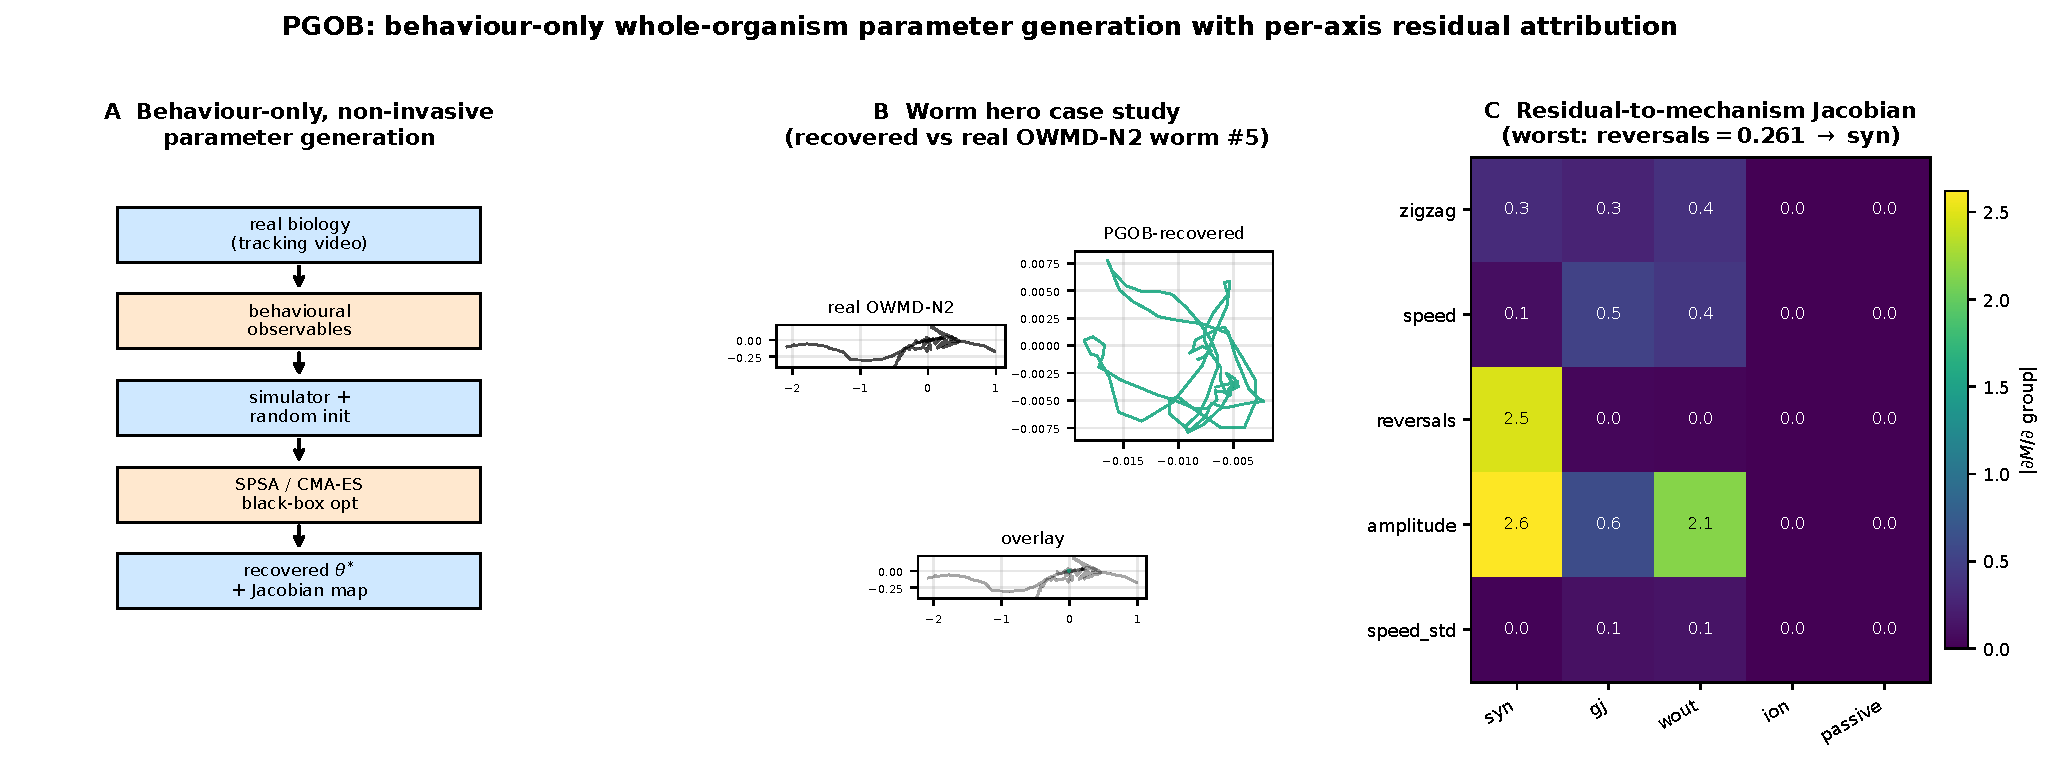
\includegraphics[width=0.95\textwidth]{Fig1_v8_composite_hero.pdf}
\caption{\textbf{PGOB: behaviour-only parameter generation with per-axis residual attribution.} \textbf{a}, Framework: tracking video $\to$ behavioural observables $\to$ simulator with random init $\to$ black-box optimiser / amortized posterior on the behavioural loss $\to$ generated $\theta^{*}$ and Jacobian attribution map (no electrophysiology at any stage). \textbf{b}, Worm case study: centreline traces of a real OWMD-N2 worm, the PGOB-generated worm, and overlay; the generated worm reproduces the travelling-wave undulation the deposited default does not. \textbf{c}, Residual-to-mechanism Jacobian at the generated BAAIWorm $\theta^{*}$: the worst per-metric residual (reversals) routes to the dominant synaptic axis.}
\label{fig:hero}
\end{figure}

\begin{figure}[H]
\centering
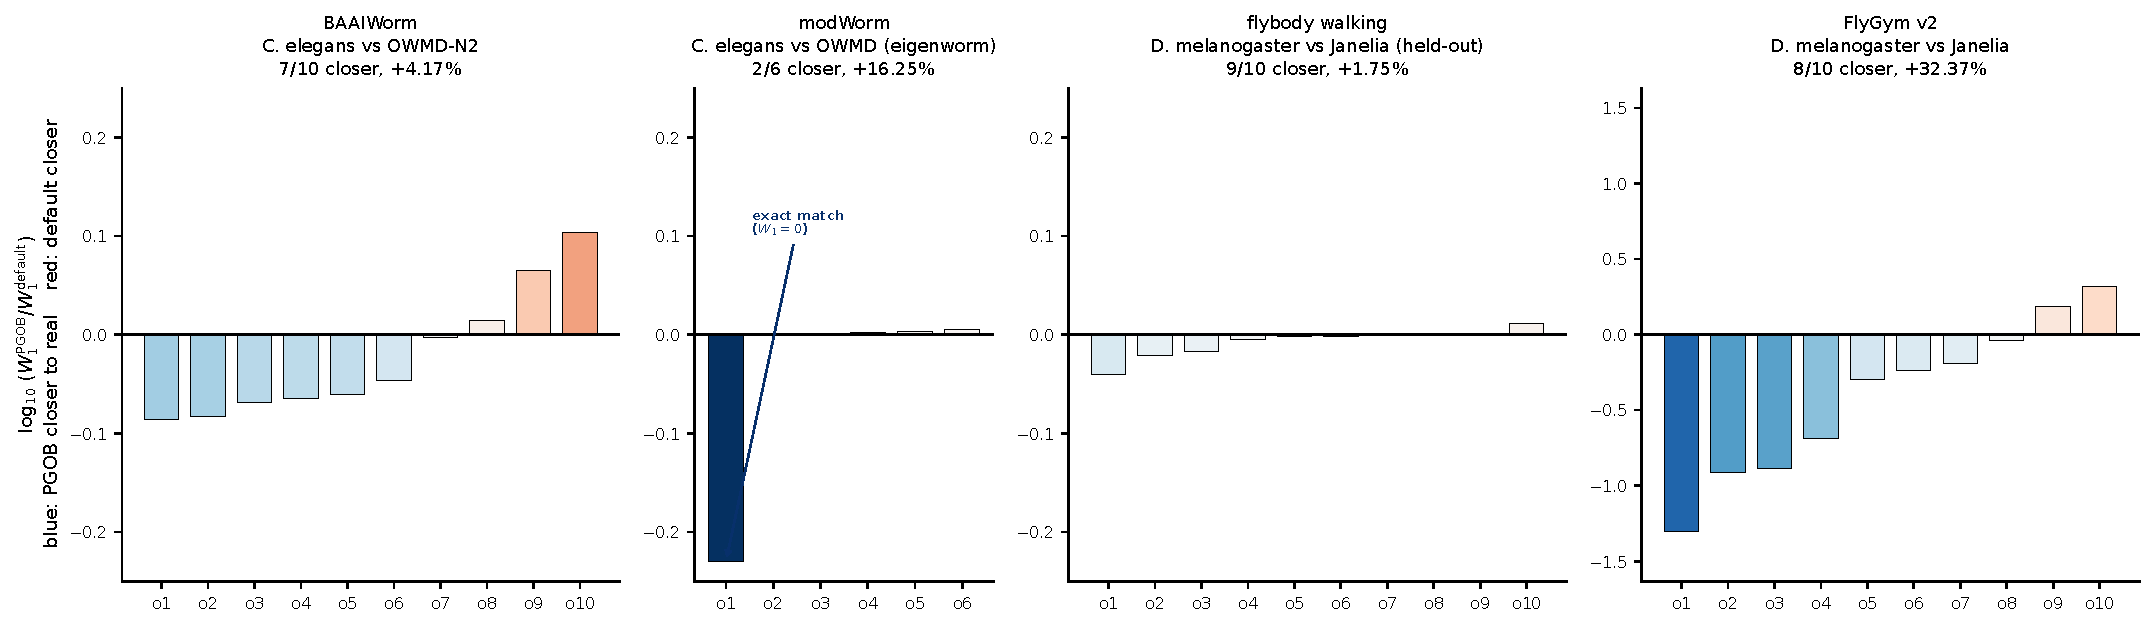
\includegraphics[width=0.95\textwidth]{Fig_HERO_1_v6.pdf}
\caption{\textbf{Per-observable PGOB-vs-baseline Wasserstein-1 across four simulators.} Each bar is $\log_{10}(W_1^{\rm PGOB}/W_1^{\rm baseline})$ for one behavioural observable; a negative (blue) bar means the generated simulator is closer to real biology. The baseline differs by panel and is labelled accordingly---an \emph{Initialized} (randomised) start for the FlyGym capability test versus an \emph{expert default} for the BAAIWorm and flybody deployment tests---so panels are not a single cross-simulator comparison. Vertical scales are per-panel and improved-observable counts are reported per simulator against its own baseline type, never summed across the heterogeneous baselines; the flybody deployment panel is a genuine null ($0/9$). The cross-simulator-comparable quantity is the three-distance hierarchy (Table~\ref{tab:hierarchy}).}
\label{fig:logratio}
\end{figure}

\begin{figure}[H]
\centering
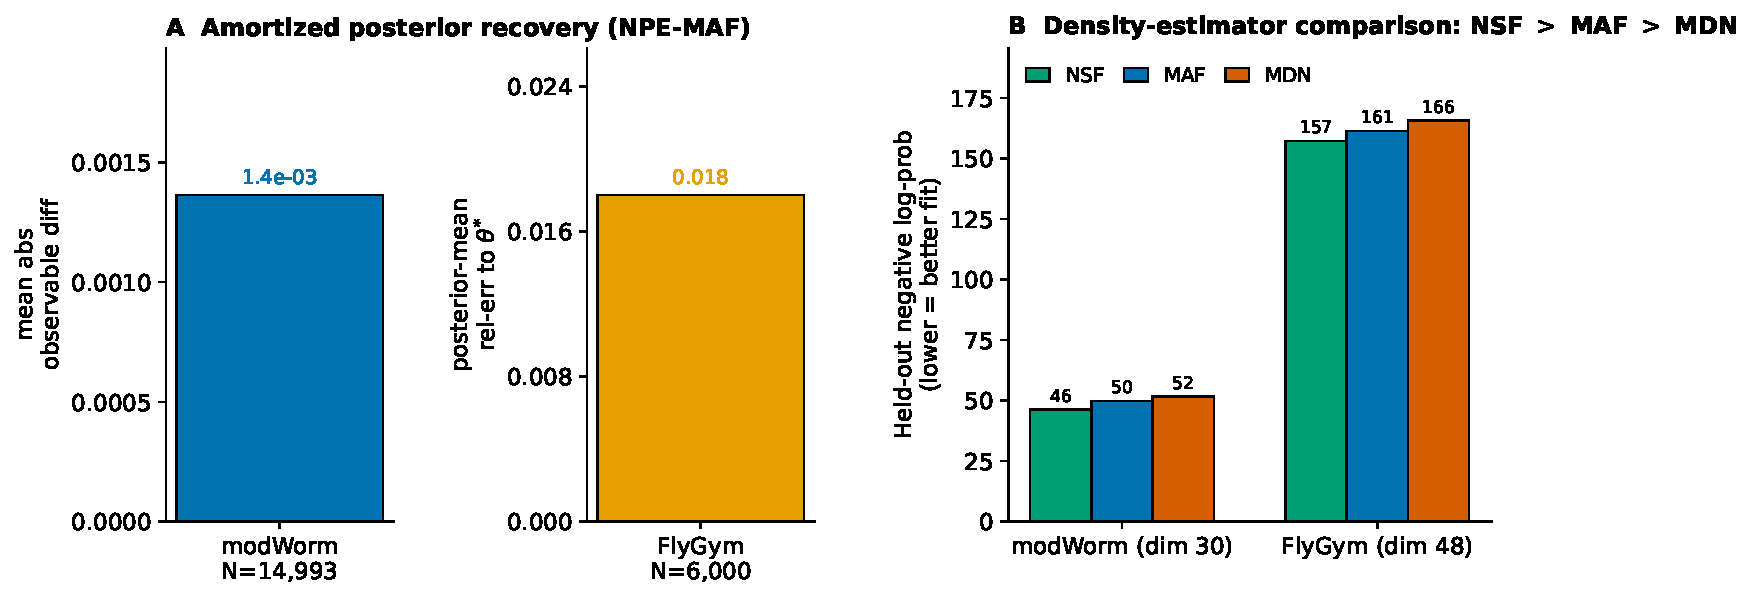
\includegraphics[width=0.95\textwidth]{Fig_sbi_engine.pdf}
\caption{\textbf{The PGOB formulation with an amortized neural-posterior engine.} \textbf{a}, Posterior-predictive reproduction of each simulator's own behaviour (modWorm mean absolute observable difference $1.4{\times}10^{-3}$; FlyGym posterior-mean $\mathrm{rel}_\theta{=}0.018$). \textbf{b}, Held-out negative log-probability for three density estimators (neural spline flow $>$ MAF $>$ mixture-density network on both simulators). The optimiser and the amortized posterior are interchangeable back-ends of one behaviour-only formulation.}
\label{fig:engine}
\end{figure}

\begin{figure}[H]
\centering
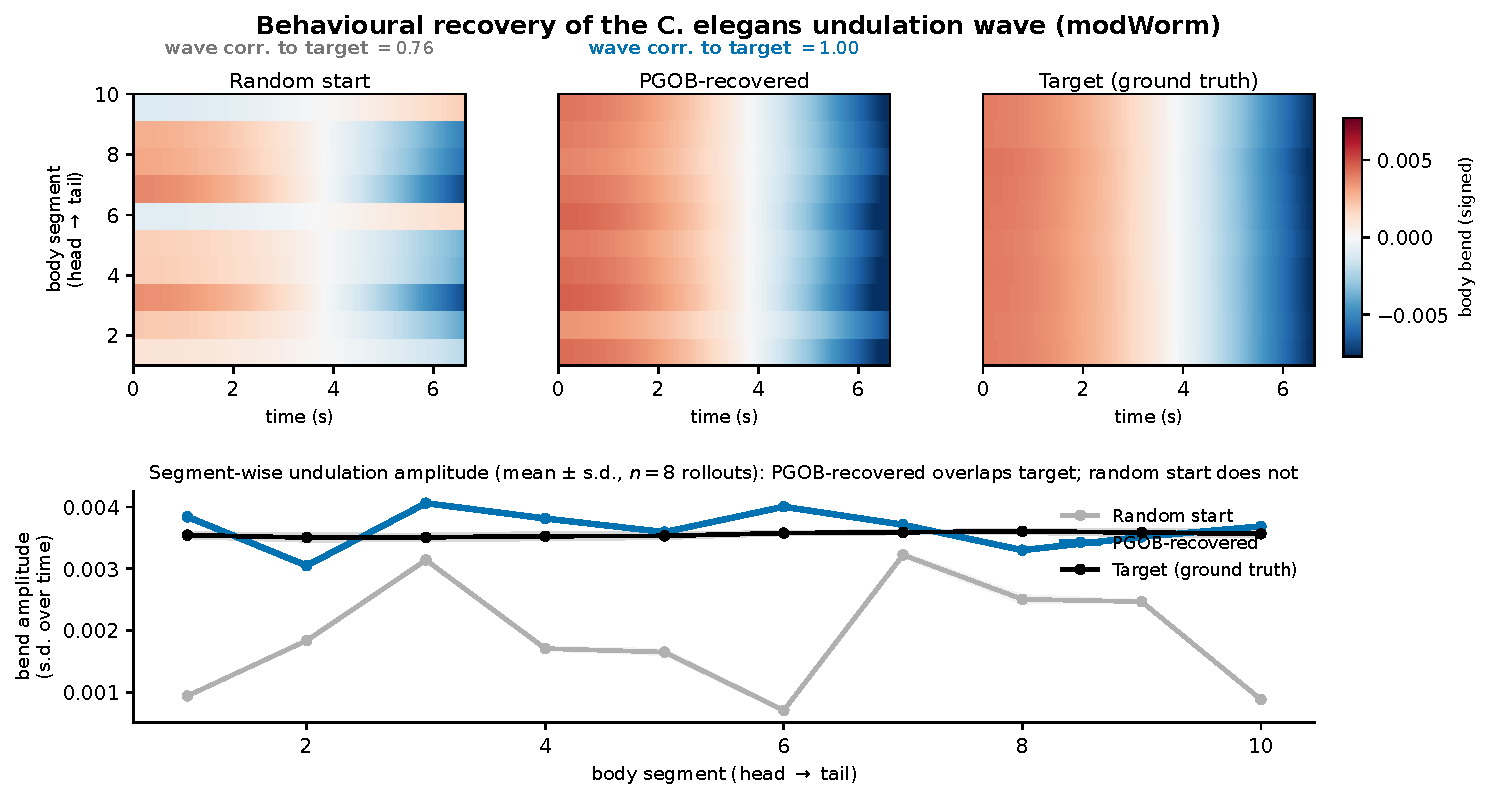
\includegraphics[width=0.8\textwidth]{Fig_worm_trajectory.pdf}
\caption{\textbf{Behaviour-level generation of the \emph{C.~elegans} undulation wave (modWorm).} Body-bend-oscillation kymographs (temporal mean removed) for a random scrambled start, the PGOB-generated parameters, and the simulator's ground-truth target ($n{=}8$ seeds each); the generated worm reproduces the travelling wave (bend-wave correlation to target $0.76\to1.00$), the random start does not. The match is behavioural: the generated parameters lie on the behaviourally-equivalent set, not necessarily at the exact ground-truth coordinates.}
\label{fig:wave}
\end{figure}

\begin{figure}[H]
\centering
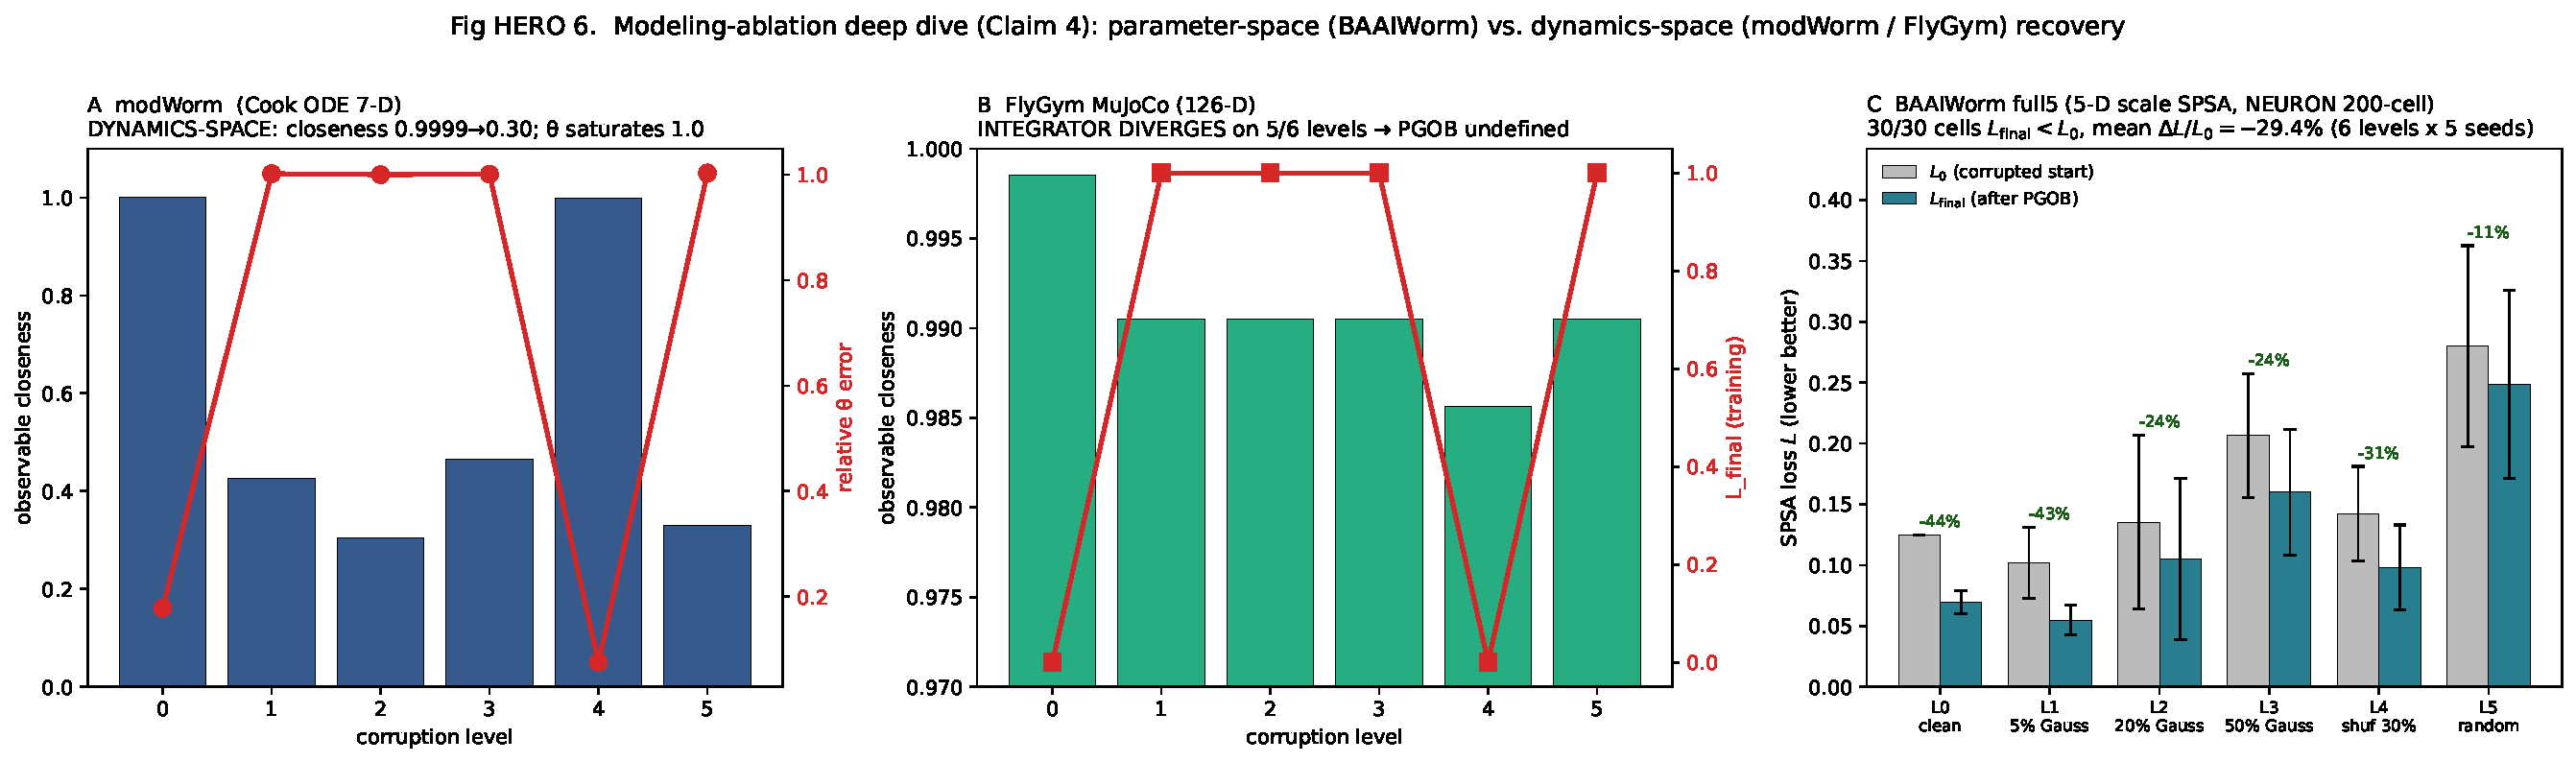
\includegraphics[width=0.95\textwidth]{Fig_HERO_6_modeling_ablation.pdf}
\caption{\textbf{Scope of PGOB: parameter-space corruption is generated back, dynamics-space corruption is not.} \textbf{a}, modWorm (Cook ODE) \emph{dynamics}-space corruption: injecting state noise collapses observable closeness from $0.9999$ to $0.30$--$0.46$ (orange; grey are intact). \textbf{b}, FlyGym v2 (MuJoCo) \emph{dynamics}-space corruption: the integrator diverges on $4/6$ levels ($L_{\rm final}{=}1.0$), leaving no usable forward model. \textbf{c}, BAAIWorm \emph{parameter}-space corruption: corrupted-start loss $L_0$ vs.\ after-PGOB loss $L_{\rm final}$ per level; $30/30$ cells improve, mean $\Delta L/L_0{=}-29.4\%$ over the full $L_0$--$L_5$ sweep. PGOB is a parameter-space generation framework, not a dynamics-space repair tool.}
\label{fig:ablation}
\end{figure}

\bibliographystyle{plainnat}
\bibliography{references}

\end{document}
